\chapter{Implementation and Development}
\label{chap:chapter4}

This chapter describes the implementation choices for the digital twin prototype: hardware assembly, geometric model construction, software architecture, and user interface. Detailed line-by-line code descriptions are omitted; only architectural decisions and technology selections are presented.

\section{Prototype Development}

The prototype corresponds to Technology Readiness Level 4, validated in a controlled environment \cite{ec2017trl}. Development followed two parallel workstreams: hardware instrumentation of the BCN3D+ printer and creation of the 3D geometric model. These were integrated at the dashboard level.

\subsection{Hardware Assembly and Sensor Node Deployment}

All components are off-the-shelf and low-cost (total under €50 \cite{shomenov2025}). The system uses:
\begin{itemize}
    \item ESP8266 NodeMCU (sensor node)
    \item MPU-6050 GY-521 (6-axis IMU) mounted on X-carriage
    \item KY-013 NTC thermistor attached to heatsink
    \item Filament encoder attached to filament between the spool and the extruder
    \item 10 k\Omega reference resistor network, breadboard, jumper wires, USB power bank
    \item Raspberry Pi (edge gateway) or laptop as alternative
\end{itemize}

The ESP8266 connects to the MPU-6050 via I²C (SDA/SCL) and to the thermistor via ADC. No wires enter the printer electronics enclosure; no firmware modifications are made \cite{esp8266_trm}. The Raspberry Pi runs OctoPrint 1.11.x, Mosquitto MQTT broker, and all Python backend scripts.

Figure~\ref{fig:uml_deployment} shows the UML Deployment Diagram of the physical infrastructure. The diagram illustrates the hardware nodes (BCN3D+ printer, ESP8266 sensor node, Raspberry Pi gateway) and the communication links between them, including I²C, ADC, USB, WiFi, and MQTT protocols.

\begin{figure}[H]
    \centering
    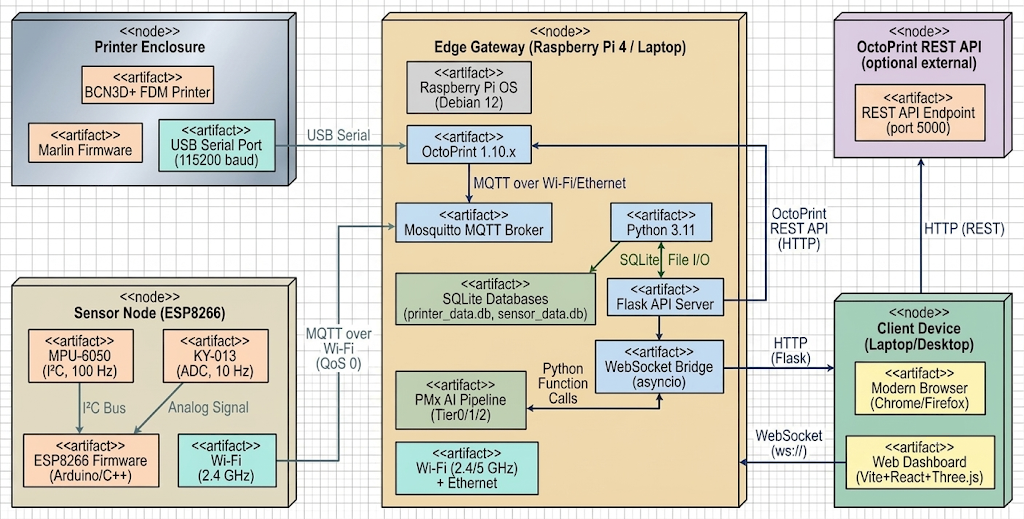
\includegraphics[width=0.9\textwidth]{figures/diagram_uml_deployment}
    \caption{UML Deployment Diagram: physical infrastructure}
    \label{fig:uml_deployment}
\end{figure}

\subsection{Geometric Model Construction: Blender Workflow}

The 3D model of the BCN3D+ was created in Blender 4.x \cite{blender2024manual}. The model uses metric units (mm) and is decomposed into named objects corresponding to FMEA components: \texttt{nozzle\_assembly}, \texttt{x\_carriage}, \texttt{x\_belt}, \texttt{extruder\_heatsink}, etc. PBR materials and six-point lighting were applied. The model is exported as glTF 2.0 binary (.glb) \cite{khronos2022gltf} and served as a static asset. At runtime, Three.js updates object positions and changes material colours for fault highlighting.

\section{Software Implementation}

The software stack follows a layered architecture: database persistence, Python backend processing, and a React/Vite/Three.js frontend.

Figure~\ref{fig:uml_component} presents the UML Component Diagram, showing the major software components and their dependencies. The diagram includes the SQLite databases (printer\_data.db and sensor\_data.db), the Python backend modules (collectors, aligner, feature engineering, PMx AI), and the frontend dashboard (React/Three.js), connected via MQTT and WebSocket bridges.

\begin{figure}[H]
    \centering
    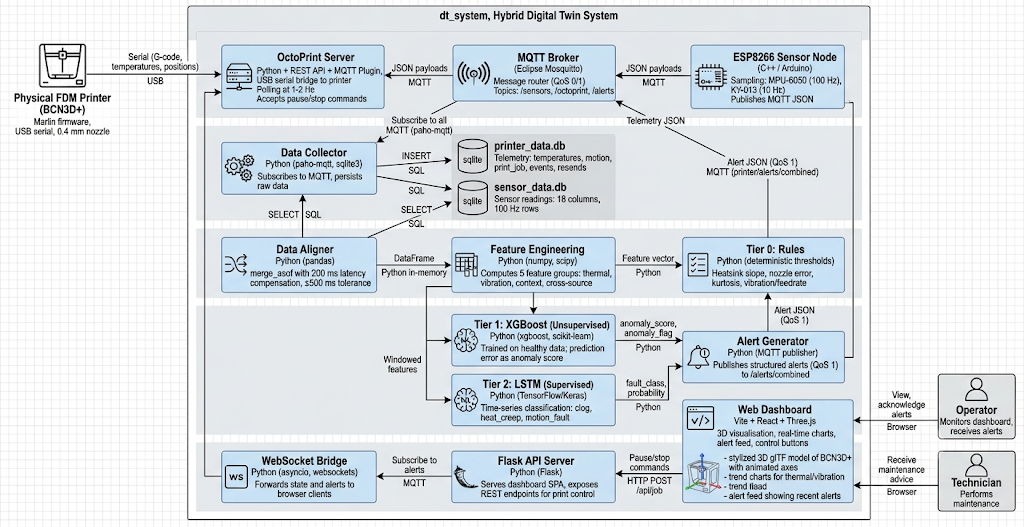
\includegraphics[width=0.9\textwidth]{figures/diagram_uml_component}
    \caption{UML Component Diagram: software and hardware components}
    \label{fig:uml_component}
\end{figure}

\subsection{Database Implementation}

Two SQLite databases store all data \cite{sqlite2024}:

\begin{itemize}
    \item \texttt{printer\_data.db}: six tables (\texttt{temperatures}, \texttt{motion}, \texttt{print\_job}, \texttt{printer\_state}, \texttt{events}, \texttt{resends}) populated from OctoPrint MQTT telemetry.
    \item \texttt{sensor\_data.db}: single table with 18 columns (timestamps, temperatures, accelerometer and gyroscope values with deltas) populated from ESP8266 MQTT payloads.
\end{itemize}

Write-Ahead Logging (WAL) is enabled to allow concurrent reads and writes. Indexes on timestamp columns enable efficient \texttt{merge\_asof} alignment.

\subsection{Python Backend Processing}

The backend consists of six scripts, but only the key architectural choices are highlighted:

\begin{itemize}
    \item \texttt{printer\_data\_collector.py} and \texttt{sensor\_data\_collector.py} subscribe to MQTT topics and insert rows into SQLite.
    \item \texttt{data\_aligner.py} shifts sensor timestamps backward by 200 ms (latency compensation) and uses Pandas \texttt{merge\_asof} with ±500 ms tolerance to align the two streams \cite{mckinney2010data}.
    \item \texttt{feature\_engineering.py} computes the five feature groups (thermal, vibration, spectral, context, cross-source). Adaptive window scaling handles insufficient data at session start.
    \item The PMx AI pipeline (Tier 0 rules, Tier 1 Isolation Forest, Tier 2 XGBoost, ensemble combiner) runs in real time. Tier 0 is fully operational; Tier 1 requires at least 10 healthy prints; Tier 2 is bootstrapping (motion fault weight set to 0.0 until sufficient data).
\end{itemize}

All divisions by zero and infinite values are replaced with 0.0 to ensure runtime stability on the Raspberry Pi.

\subsection{User Interface: Web Dashboard}

The dashboard is a single-page application built with Vite, React (TypeScript), and Three.js \cite{pmc2025building}. It is accessible at \texttt{http://<device-ip>:5000} with no installation.

\subsubsection{Frontend Architecture}
The codebase is modular:
\begin{itemize}
    \item \texttt{scene/}: Three.js setup (camera, lighting, renderer)
    \item \texttt{model/}: GLB loader and named-part registry
    \item \texttt{printer\_manager/motion/}: axis motion classes (X, Y, Z)
    \item \texttt{gcode/}: G-code parser and path generators
    \item \texttt{visualization/}: \texttt{FilamentRenderer} for live filament path
    \item \texttt{src/providers/}: \texttt{StandaloneProvider} (local G-code playback) and \texttt{StreamProvider} (MQTT stream consumer) – both implement the same interface, decoupling data source from rendering.
\end{itemize}

The \texttt{StreamProvider} filters motion packets (checks for valid \texttt{x\_mm} and \texttt{y\_mm}) to avoid snapping the virtual head to (0,0,0) on non-motion updates.

Figure~\ref{fig:blender_glb_model} shows the imported GLB printer model as visualized in Blender during the modeling phase. The image highlights the component decomposition and material assignments.

\begin{figure}[H]
    \centering
    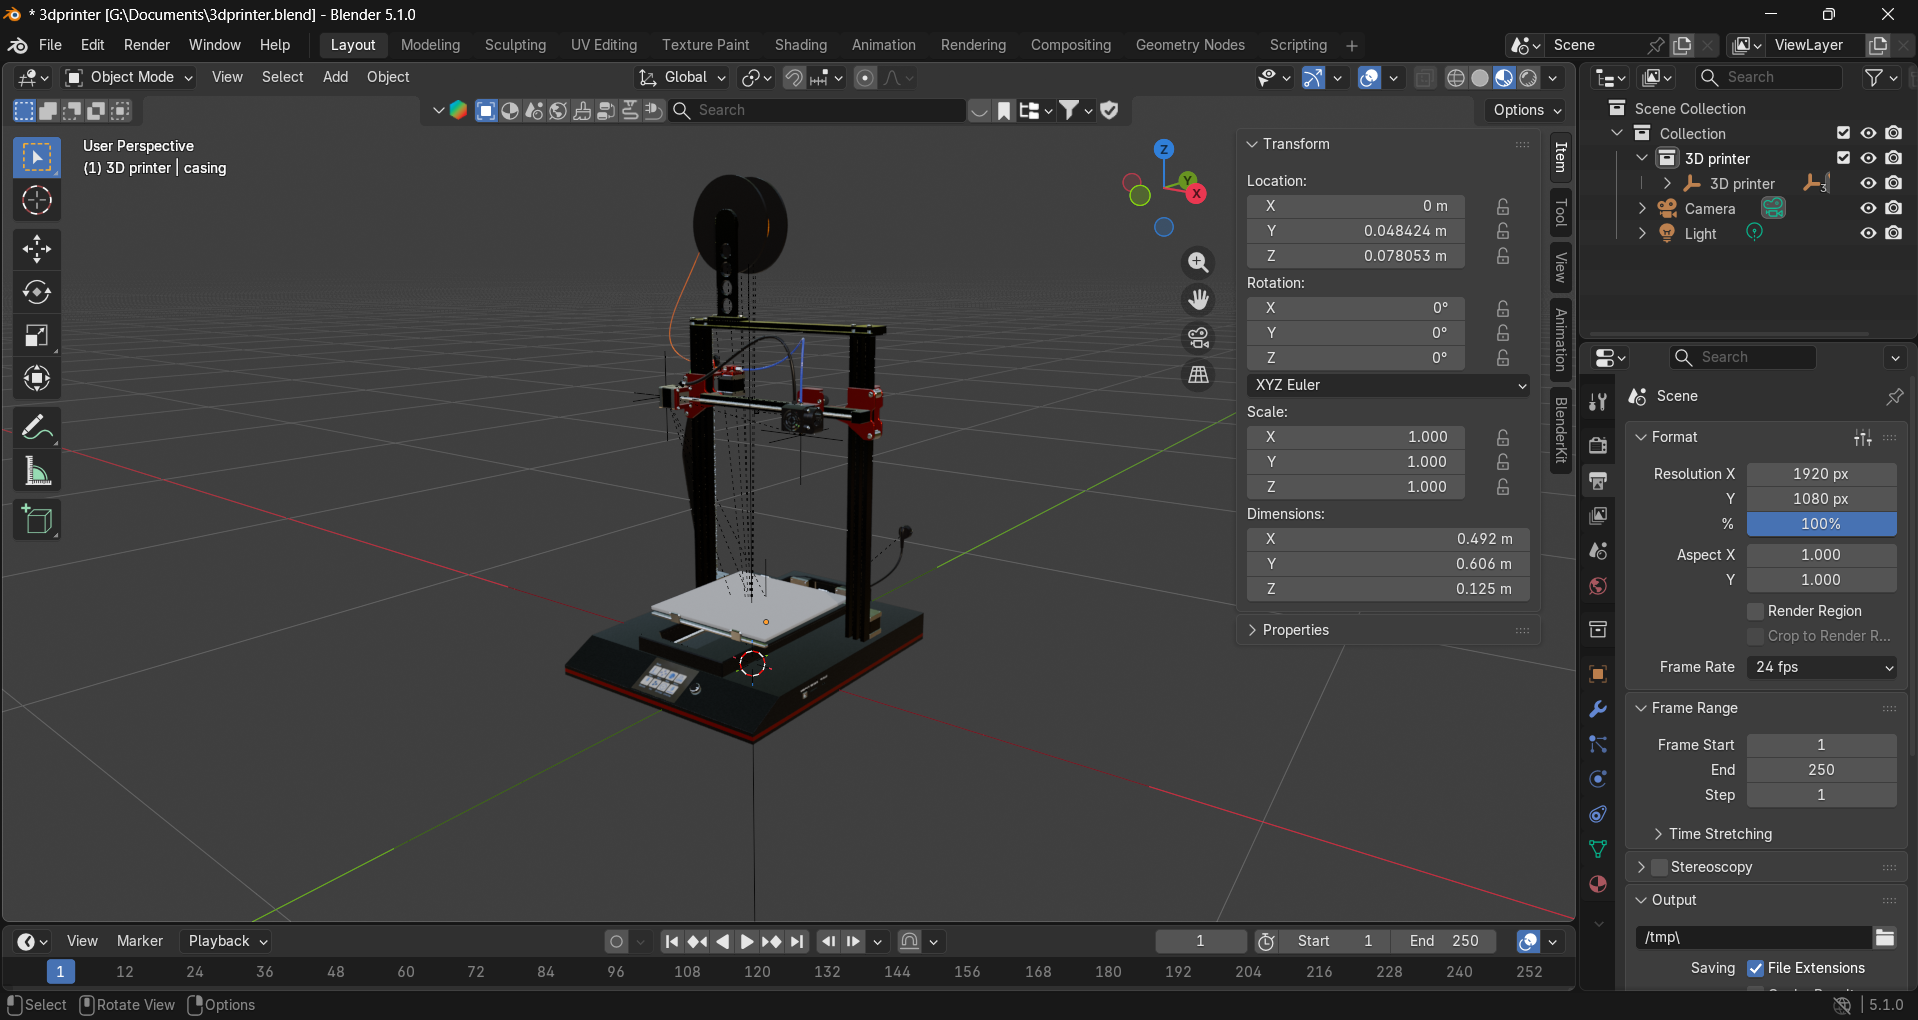
\includegraphics[width=0.85\textwidth]{figures/figure_blender_glb_model.png}
    \caption{Imported GLB printer model visualized in Blender.}
    \label{fig:blender_glb_model}
\end{figure}

Figure~\ref{fig:standalone_mode} presents the standalone mode interface, which supports local G-code playback without requiring a live printer connection. This mode is useful for testing and demonstration purposes.

\begin{figure}[H]
    \centering
    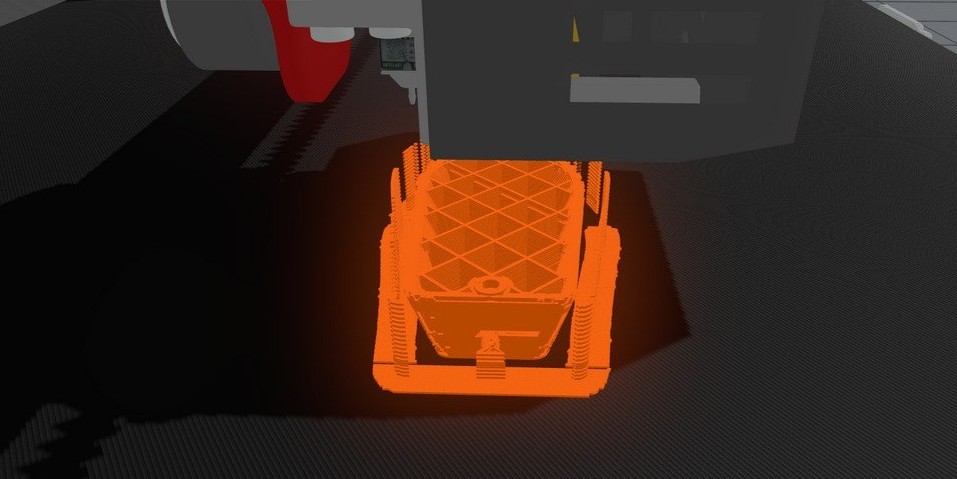
\includegraphics[width=0.85\textwidth]{figures/figure_standalone_mode.jpg}
    \caption{Standalone mode interface showing local G-code playback capabilities.}
    \label{fig:standalone_mode}
\end{figure}

Figure~\ref{fig:stream_mode} shows the stream mode interface, which displays real-time MQTT data visualization during active printer operation. The interface shows live sensor readings and axis positions.

\begin{figure}[H]
    \centering
    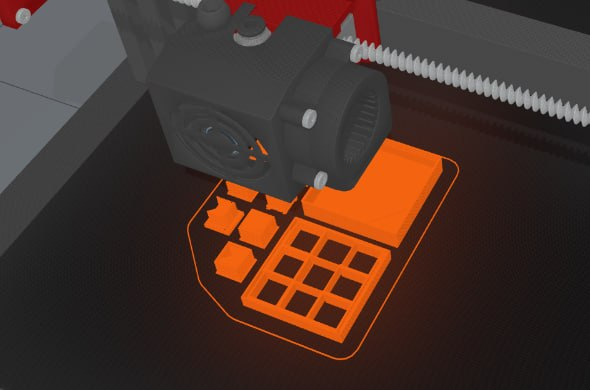
\includegraphics[width=0.85\textwidth]{figures/figure_stream_mode.jpg}
    \caption{Stream mode interface showing real-time MQTT data visualization.}
    \label{fig:stream_mode}
\end{figure}

\subsubsection{3D Visualisation and Fault Overlays}
Axis positions received via MQTT WebSocket are applied to Three.js meshes using \texttt{Object3D.position.set()}. The \texttt{FilamentRenderer} appends points on extrusion moves (G1 with positive E delta) and inserts break points on travel moves (G0). When an alert is generated, the backend pushes a structured JSON object.

\subsubsection{Alert System and Dashboard Layout}
The dashboard has three panels: central 3D canvas, left sensor charts (thermal and vibration), and right alert feed. Alerts contain timestamp, fault class, severity, triggering signal, component ID, and recommended action. CRIT alerts automatically send a print pause command via OctoPrint REST API (\texttt{POST /api/job} with \texttt{\{"command": "pause"\}}).

\subsection{Desktop Application}

An Electron.js wrapper is under development \cite{electron2024}. It reuses the same React/Vite/Three.js codebase and adds native features (file system, system tray). The desktop version shares the same Flask backend and WebSocket bridge, requiring no code duplication.

Figure~\ref{fig:dashboard_overview} presents the main dashboard overview. The dashboard integrates the digital twin visualization (center), machine status indicators and sensor monitoring panels (left), and predictive maintenance metrics and alerts (right). The 3D printer model updates its position in real time based on incoming MQTT telemetry.

\begin{figure}[H]
    \centering
    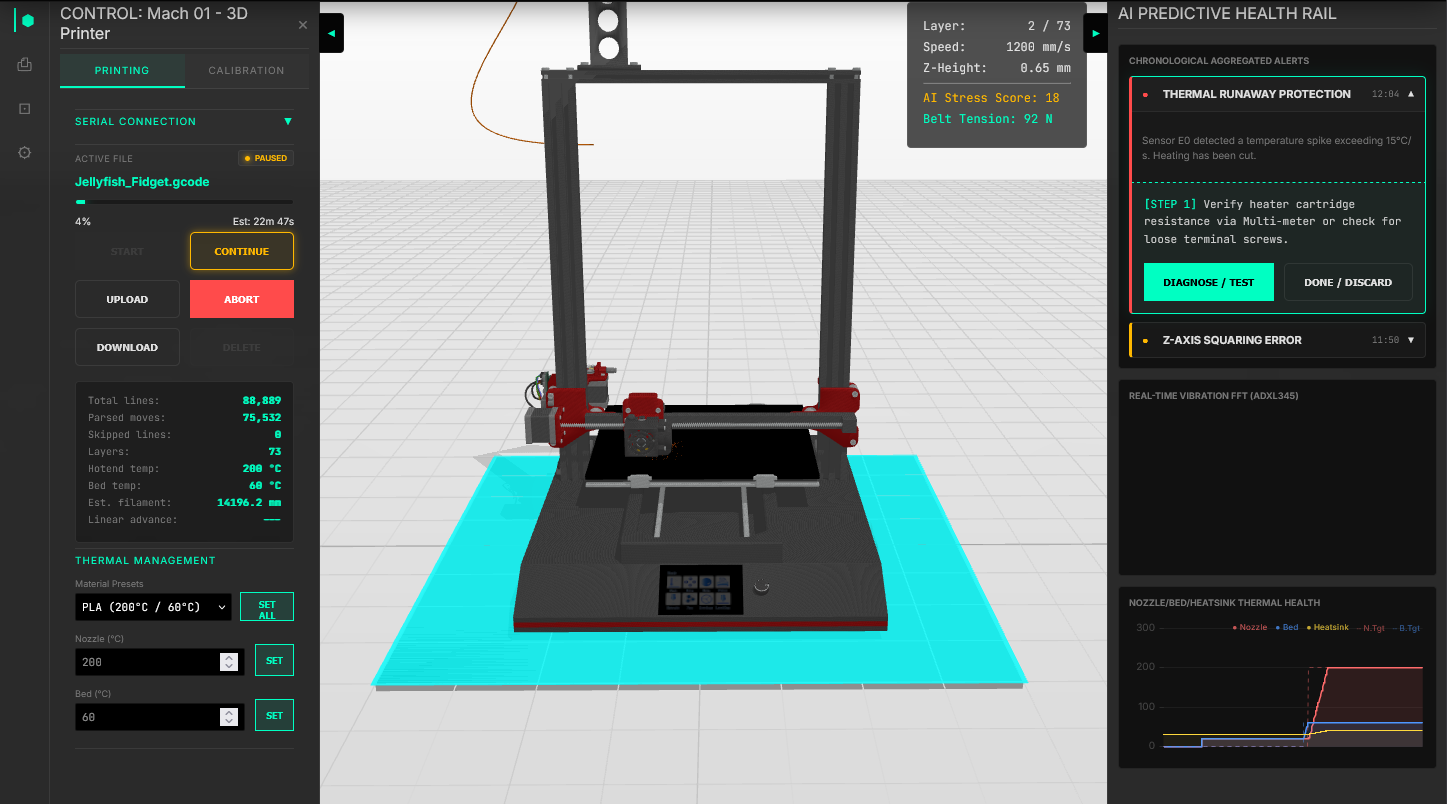
\includegraphics[width=\textwidth]{figures/figure_dashboard_screenshot.png}
    \caption{Main dashboard overview showing the digital twin visualization, machine status indicators, sensor monitoring panels, and predictive maintenance metrics.}
    \label{fig:dashboard_overview}
\end{figure}

\section{Summary of Implementation Choices}

The prototype is built on open-source, low-cost technologies: ESP8266 for sensing, MQTT for communication, SQLite for persistence, Python for data alignment and ML, and Three.js for visualisation. The architecture is edge-first (no cloud dependency) and requires no firmware modification, ensuring transferability to any OctoPrint-managed FDM printer.

\endinput